\documentclass[12pt,a4paper]{article} % fleqn
\usepackage{cite}
\usepackage{enumitem}
\usepackage{latexsym}
\usepackage{graphicx}
\usepackage{iman}
\usepackage{extra}
\usepackage{isar}
\usepackage{isabelle}
\usepackage{isabellesym}
\usepackage{style}
\usepackage{pdfsetup}
\usepackage{railsetup}
\usepackage{framed}

\newbox\boxA
\setbox\boxA=\hbox{\ }
\parindent=4\wd\boxA

\newcommand{\keyw}[1]{\isacommand{#1}}

\renewcommand{\isactrlsub}[1]{\/$\sb{\mathrm{#1}}$}
\renewcommand{\isacharprime}{\isamath{{'}\mskip-2mu}}
\renewcommand{\isacharunderscore}{\mbox{\_}}
\renewcommand{\isacharunderscorekeyword}{\mbox{\_}}
\renewcommand{\isachardoublequote}{\mbox{\upshape{``}}}
\renewcommand{\isachardoublequoteopen}{\mbox{\upshape{``}\kern.1ex}}
\renewcommand{\isachardoublequoteclose}{\/\kern.15ex\mbox{\upshape{''}}}

\hyphenation{isa-belle}

\isadroptag{theory}

\title{%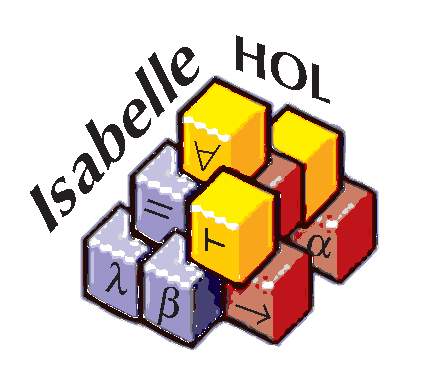
\includegraphics[scale=0.5]{isabelle_hol} \\[4ex]
Defining (Co)datatypes in Isabelle/HOL}
\author{\hbox{} \\
Jasmin Christian Blanchette \\
Lorenz Panny \\
Andrei Popescu \\
Dmitriy Traytel \\
{\normalsize Institut f\"ur Informatik, Technische Universit\"at M\"unchen} \\
\hbox{}}
\begin{document}

\maketitle

\begin{abstract}
\noindent
This tutorial describes how to use the new package for defining datatypes and
codatatypes in Isabelle/HOL. The package provides four main user-level commands:
\keyw{datatype\_new}, \keyw{codatatype}, \keyw{primrec\_new}, and \keyw{primcorec}.
The commands suffixed by \keyw{\_new} are intended to subsume, and eventually
replace, the corresponding commands from the old datatype package.
\end{abstract}

\tableofcontents

\input{Datatypes.tex}

\let\em=\sl
\bibliography{manual}{}
\bibliographystyle{abbrv}

\end{document}
